% cspc-internals.tex — The cspc Compiler: Internal Architecture
% April 14, 2026
\documentclass[11pt,letterpaper]{article}

\usepackage[margin=1in]{geometry}
\usepackage{amsmath,amssymb}
\usepackage{booktabs}
\usepackage{longtable}
\usepackage{listings}
\usepackage{xcolor}
\usepackage{tikz}
\usetikzlibrary{arrows.meta,positioning,fit}
\usepackage{enumitem}
\usepackage[colorlinks=true,linkcolor=blue,citecolor=blue,urlcolor=blue]{hyperref}

\lstdefinelanguage{Scheme}{
  morekeywords={define,lambda,let,let*,letrec,if,cond,case,else,begin,do,
    set!,car,cdr,cons,map,filter,apply,error,and,or,not,eq?,equal?,
    display,newline},
  sensitive=true,
  morecomment=[l]{;},
  morestring=[b]",
  basicstyle=\ttfamily\footnotesize,
  keywordstyle=\bfseries\color{blue!60!black},
  commentstyle=\itshape\color{gray},
  showstringspaces=false,
  columns=flexible,
  breaklines=true,
  numbers=left,
  numberstyle=\tiny\color{gray},
  numbersep=5pt,
  xleftmargin=1.5em
}
\lstset{language=Scheme}

\title{The \texttt{cspc} Compiler:\\
  Internal Architecture and Compilation Pipeline}
\author{Mika Nystr\"om}
\date{April 14, 2026}

\begin{document}
\maketitle
\tableofcontents
\newpage

% ============================================================
\section{Overview}

\texttt{cspc} is a compiler from Fulcrum-CSP (FCSP), Intel's dialect of
Martin's Communicating Sequential Processes for hardware design (CSP), to compiled Modula-3
executables.  The compiled output links against \texttt{cspsimlib}, a
cooperative-scheduling runtime library that implements channels,
processes, and the CSP rendezvous semantics.

The compiler is written in Scheme (approximately 17,200~lines across
48~modules in \texttt{csp/src/}) and runs inside the \texttt{mscheme}
interpreter embedded in Modula-3.  The compiler generates Modula-3
source code directly; the generated code is then compiled by
\texttt{cm3} and linked against the \texttt{cspsimlib} runtime.
The resulting executables achieve over 200,000 simulated instructions
per second on an ARM processor using the C-based Modula-3 back end.
This figure is for a \emph{decomposed} design: the full 32-bit
MiniMIPS pipelined processor (seven or eight concurrent processes
communicating via channels), not a simple sequential program.  The
scheduler sustains approximately 9~million context switches per
second---each ``switch'' is simply a procedure return followed by a
procedure call through a continuation pointer, with no stack
save/restore or OS involvement.  On an x86-64 server with the
GCC-based Modula-3 back end (which generates assembly directly,
avoiding the extra C compilation layer), throughput would
approximately double.

\subsection{The Big Picture}

The compilation pipeline has three major phases:

\begin{center}
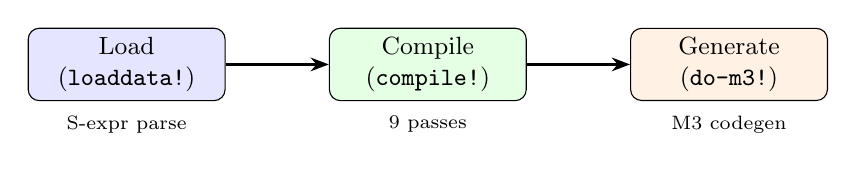
\begin{tikzpicture}[>=Stealth, scale=0.85,
    phase/.style={draw, rounded corners, minimum width=2.5cm,
      minimum height=0.8cm, font=\small, align=center},
    arr/.style={->, thick}]
  \node[phase, fill=blue!10] (load) at (0,0) {Load\\(\texttt{loaddata!})};
  \node[phase, fill=green!10] (comp) at (4.5,0) {Compile\\(\texttt{compile!})};
  \node[phase, fill=orange!10] (gen) at (9,0) {Generate\\(\texttt{do-m3!})};
  \draw[arr] (load) -- (comp);
  \draw[arr] (comp) -- (gen);
  \node[below=2pt of load, font=\scriptsize] {S-expr parse};
  \node[below=2pt of comp, font=\scriptsize] {9 passes};
  \node[below=2pt of gen, font=\scriptsize] {M3 codegen};
\end{tikzpicture}
\end{center}

\begin{enumerate}[nosep]
  \item \textbf{\texttt{loaddata!}} reads the S-expression intermediate
    form from disk (originally produced by a Java parser).
  \item \textbf{\texttt{compile!}} runs nine transformation passes
    (\texttt{compile1!} through \texttt{compile9!}).
  \item \textbf{\texttt{do-m3!}} generates Modula-3 source, an
    \texttt{m3makefile}, and builds the executable via \texttt{cm3}.
\end{enumerate}

The result is a standalone executable that simulates the CSP design
at compiled speed.

\subsection{Source Organization}

\begin{center}
\begin{tabular}{llr}
\toprule
\textbf{Directory} & \textbf{Purpose} & \textbf{Lines} \\
\midrule
\texttt{csp/src/} & Compiler (Scheme) & 17,193 \\
\texttt{csp/cspsimlib/src/} & Runtime library (M3) & 2,412 \\
\texttt{csp/cspgrammar/src/} & AST types (M3) & 1,788 \\
\midrule
\textbf{Total} & & \textbf{21,393} \\
\bottomrule
\end{tabular}
\end{center}

The largest single module is \texttt{codegen-m3.scm} at 4,241~lines,
which generates the Modula-3 output.  The main compiler driver is
\texttt{cspc.scm} at 1,663~lines.


% ============================================================
\section{The Compilation Pipeline}
\label{sec:pipeline}

The compiler transforms CSP source through nine numbered passes.
Each pass is defined in \texttt{passes.scm} and stores its result
in a global variable (\texttt{text1} through \texttt{text9}).

\subsection{Pass 1: Loop Uniquification (\texttt{compile1!})}

Renames loop iteration variables to ensure each loop body has unique
variable names.  This prevents name collisions when loops are unrolled
or parallelized in later passes.

\begin{lstlisting}
(define (compile1!)
  (set! text1 (uniquify-loop-dummies *the-text*))
  'text1)
\end{lstlisting}

\subsection{Pass 2: Core Transformations (\texttt{compile2!})}

The largest pass, comprising 16 sub-passes run to a fixed point:

\begin{center}
\begin{tabular}{ll}
\toprule
\textbf{Sub-pass} & \textbf{Purpose} \\
\midrule
\texttt{handle-access-assign} & Resolve struct/array access on LHS \\
\texttt{handle-access-recv} & Resolve struct/array in receive/send \\
\texttt{handle-assign-rhs} & Expression sequencing on assignment RHS \\
\texttt{handle-send-rhs} & Expression sequencing on send value \\
\texttt{handle-eval} & Evaluate constant expressions \\
\texttt{inline-evals} & \textbf{Function inlining} \\
\texttt{handle-assign-shortcircuit} & Short-circuit boolean assignment \\
\texttt{global-simplify} & Statement simplification \\
\texttt{remove-assign-operate} & Remove \texttt{x += c} $\to$ \texttt{x = x + c} \\
\texttt{remove-do} & Desugar \texttt{do} loops \\
\texttt{remove-choose} & Desugar choose expressions \\
\texttt{simplify-if} & Simplify trivial if guards \\
\texttt{convert-waiting-ifs} & Convert blocking ifs to waiting form \\
\texttt{unfold-loop-ranges} & Expand loop range expressions \\
\texttt{remove-loop-expression} & Desugar loop expressions on LHS \\
\bottomrule
\end{tabular}
\end{center}

The sub-passes are applied repeatedly until no further changes occur
(fixed-point iteration).  Function inlining (\texttt{inline-evals})
is the most complex sub-pass and is described in
Section~\ref{sec:inline}.

\subsection{Pass 3: Struct Conversion + Constant Folding (\texttt{compile3!})}

\begin{enumerate}[nosep]
  \item Convert struct send/receive operations into pack/unpack
    sequences (\texttt{convert-send-struct}, \texttt{convert-recv-struct}).
  \item Fold constant expressions (\texttt{fold-constants-*}).
\end{enumerate}

\subsection{Pass 4: Constant Propagation (\texttt{compile4!})}

\begin{enumerate}[nosep]
  \item Patch uninitialized variable uses.
  \item Fold remaining constants.
  \item Identify and promote constant variables
    (\texttt{constantify-constant-vars}).
\end{enumerate}

\subsection{Pass 5: Parallel and Loop Optimization (\texttt{compile5!})}

\begin{enumerate}[nosep]
  \item Sequentialize non-blocking parallel compositions (if both
    branches are non-blocking, convert \texttt{A,B} to \texttt{A;B}).
  \item Delete unused variables.
  \item Simplify statements.
  \item Unroll parallel loops.
  \item Unblock sequential loops (convert loop bodies that never
    block into simple M3 loops).
\end{enumerate}

\subsection{Pass 6: Type Analysis and Interval Arithmetic (\texttt{compile6!})}

This is the most analytically sophisticated pass:

\begin{enumerate}[nosep]
  \item Merge global initializations with the program text.
  \item Insert pack/unpack copies for struct operations.
  \item Build the variable and type tables (\texttt{make-the-tables}).
  \item \textbf{Seed integer ranges} from declarations and constants.
  \item \textbf{Close integer ranges} by propagating ranges through
    all operations to a fixed point.
  \item \textbf{Propose types} --- choose the narrowest M3 type that
    covers each variable's range (Section~\ref{sec:interval}).
\end{enumerate}

\subsection{Pass 7: Block Label Insertion (\texttt{compile7!})}

Insert labels at every potential blocking point (channel operations,
probe-based selections).  These labels become the entry points of
the ``blocks'' in the compiled code.

\subsection{Pass 8: Block Extraction (\texttt{compile8!})}

Split the program into \emph{basic blocks} separated by blocking
points.  Each block is a sequence of non-blocking statements that
runs atomically.  The result is a list of blocks, each starting with
a label and ending with a goto.

This is the \texttt{scan-stmt} function from \texttt{blocking.scm}
(Section~\ref{sec:blocking}).

\subsection{Pass 9: Cleanup (\texttt{compile9!})}

Remove empty blocks and produce the final program listing.

\subsection{After the Passes: Code Generation}

After \texttt{compile!}, the program is a graph of basic blocks.
Each block is a segment of sequential code between two channel
operations (sends, receives, or selections with communication).
Channel operations are the \emph{only} points where control
leaves the process; between them, the code is straight-line
Modula-3.

\texttt{do-m3!} (in \texttt{codegen-m3.scm}) converts this block
graph to Modula-3 as follows:

\begin{itemize}[nosep]
\item Each basic block becomes a Modula-3 \textbf{procedure}.  The
  procedure body is ordinary sequential M3 code: assignments,
  conditionals, array accesses, arithmetic.
\item At the end of each block, the procedure calls the runtime to
  perform the channel operation (send or receive).  The runtime
  records which block to execute \emph{next} (the continuation)
  and returns control to the scheduler.
\item When the channel rendezvous completes (the partner process has
  executed the matching operation), the scheduler resumes the
  process by calling the next block's procedure.
\item There is no thread switching, no stack save/restore, no
  context switch in the OS sense.  The ``scheduler'' is simply a
  loop that calls M3 procedures.  Each procedure runs to
  completion (up to the next channel operation), records its
  continuation, and returns.
\item The process state (local variables) is stored in a
  heap-allocated frame object, not on the M3 call stack.  This
  allows the scheduler to interleave processes without stack
  manipulation.
\end{itemize}

The result is a graph of M3 procedures connected by continuation
pointers, driven by a simple dispatch loop.  This architecture
avoids all interpretation overhead: the inner loop of each process
is compiled, optimized M3 code.

\texttt{do-m3!} also generates the process class (which holds the
frame and continuation state), the \texttt{m3makefile}, and
optionally runs \texttt{cm3} to produce the executable.


% ============================================================
\section{The Key Subsystems}
\label{sec:subsystems}

\subsection{Function Inlining}
\label{sec:inline}

\textbf{Module}: \texttt{inline.scm} (254~lines) + \texttt{functions.scm}
(90~lines).

CSP functions must be inlined because they can contain blocking
operations (sends, receives, selections).  A CSP ``function'' is
really a macro with copy-in/copy-out semantics, similar to Verilog
tasks.

The inliner (\texttt{inline-evals}) works as follows:

\begin{enumerate}[nosep]
  \item For each function call in the AST, look up the function body
    in the function table.
  \item For each formal parameter:
    \begin{itemize}[nosep]
      \item If the direction is \texttt{in}: generate a copy-in
        assignment (\texttt{copyin-id := actual}).
      \item If \texttt{out} or \texttt{inout}: generate both copy-in
        and copy-out assignments.
    \end{itemize}
  \item Rename all local variables in the function body to avoid
    name collisions (append a unique suffix).
  \item Substitute the function body into the call site, wrapped
    in the copy-in/copy-out assignments.
\end{enumerate}

\textbf{Restrictions}: no recursion (functions are inlined
statically), no static variables (all state is in process-level
variables or channel data).

\subsection{Interval Arithmetic}
\label{sec:interval}

\textbf{Module}: \texttt{interval.scm} (453~lines) +
\texttt{integer-types.scm} (105~lines).

The interval arithmetic subsystem computes the range of every
integer variable and sub-expression in the program.  This enables
the compiler to choose the narrowest Modula-3 integer type for each
variable, which is critical for performance (64-bit arithmetic is
2--4$\times$ slower than 32-bit on most platforms).

The key function is \texttt{expr-range}, which computes the range
of an expression given the ranges of its operands:

\begin{lstlisting}
(define (expr-range expr syms)
  (cond ((bigint? expr) (make-point-range expr))
        ((ident? expr)
         (let* ((rng (search-range *the-rng-tbl* id))
                (dcl (search-range *the-dcl-tbl* id))
                (glb (search-range *the-global-ranges* id)))
           (range-intersection rng dcl glb)))
        ((binary-expr? expr)
         (let* ((op (car expr))
                (rop (eval (symbol-append 'range- op))))
           (rop (expr-range (cadr expr) syms)
                (expr-range (caddr expr) syms))))
        ...))
\end{lstlisting}

The range operations (\texttt{range-+}, \texttt{range-*},
\texttt{range-\&}, etc.) implement interval arithmetic for each
CSP operator.  Bitwise operations require special handling:
\texttt{range-\&} computes the tightest interval for $[a,b]
\mathbin{\&} [c,d]$, which is non-trivial for arbitrary intervals.

The analysis proceeds in three phases (Pass~6):
\begin{enumerate}[nosep]
  \item \textbf{Seed}: initialize ranges from type declarations
    (e.g., \texttt{int(8)} $\Rightarrow$ $[0, 255]$).
  \item \textbf{Close}: propagate ranges through all statements
    to a fixed point.
  \item \textbf{Propose}: choose the narrowest M3 type for each
    variable (\texttt{INTEGER}, \texttt{Ctypes.int\_32}, etc.).
\end{enumerate}

\subsection{Blocking Analysis}
\label{sec:blocking}

\textbf{Module}: \texttt{blocking.scm} (682~lines).

The blocking analysis determines which statements can \emph{block}
--- that is, suspend the process waiting for a communication partner.
This is the key analysis that enables efficient compilation: blocks
of non-blocking code can run as ordinary sequential M3 code, while
blocking points become process suspension/resumption points.

A statement may block if it contains:
\begin{itemize}[nosep]
  \item A \textbf{receive} (\texttt{X?y}) --- waits for a sender.
  \item A \textbf{send} (\texttt{X!e}) --- waits for a receiver.
  \item A \textbf{wait} (\texttt{wait(n)}) --- timed suspension.
  \item A \textbf{selection with probes} --- waits for channel state.
  \item An \textbf{apply} (function call that hasn't been inlined).
\end{itemize}

The function \texttt{stmt-may-block?} walks the AST and returns
\texttt{\#t} if any sub-statement or sub-expression can block:

\begin{lstlisting}
(define (stmt-may-block? stmt)
  (define result #f)
  (define (s-visitor s)
    (case (get-stmt-type s)
      ((recv send waitfor)       (set! result #t) 'cut)
      ((if nondet-if waiting-if) (set! result #t) 'cut)
      (else                      s)))
  (visit-stmt stmt s-visitor x-visitor identity)
  result)
\end{lstlisting}

The analysis then splits the program into basic blocks: each block
starts at a potential blocking point and contains only non-blocking
statements thereafter.  The blocks become the ``states'' of the
compiled process's state machine.

\textbf{Non-blocking parallel optimization}: if both branches of a
parallel composition (\texttt{A,B}) are non-blocking, the parallel
is converted to sequential (\texttt{A;B}).  This avoids the overhead
of forking and joining threads.

\subsection{Selection Compilation}
\label{sec:selection}

\textbf{Module}: \texttt{selection.scm} (439~lines) +
\texttt{choose.scm} (46~lines).

CSP selections (\texttt{[~G1 -> S1 [] G2 -> S2~]}) are the most
complex construct to compile.  The compiler distinguishes two cases:

\begin{description}[style=nextline]
  \item[Local selection]
    All guards are local expressions (no probes).  Compiled as a
    simple \texttt{IF ... ELSIF ... ELSE} chain in M3.  No blocking.

  \item[Waiting selection]
    At least one guard involves a channel probe.  Compiled as a
    state machine that evaluates guards, registers for wake-up on
    probe changes, and suspends until a guard becomes true.
\end{description}

The decision is made by \texttt{make-selection-implementation}:

\begin{lstlisting}
(define (make-selection-implementation selection ...)
  (let* ((guards (map car gcs))
         (sensitivities (map expr-sensitivity guards))
         (local (or last-guard-is-else
                    (null? (apply append sensitivities)))))
    (if local
        (implement-local-if selection ...)
        (implement-waiting-if selection ...))))
\end{lstlisting}

The ``else'' guard is handled specially: if the last guard is
\texttt{else}, the selection is always local (the else branch
catches all cases, so no blocking is needed).

\subsection{Loop Compilation}

\textbf{Module}: \texttt{loops.scm} (185~lines).

CSP's \texttt{*[~...~]} (infinite loop) compiles to a label at the
top of the loop body with a goto at the bottom.  If the loop body
contains blocking points, the loop becomes part of the block
structure (the top-of-loop label is a block entry point).

Non-blocking loops (where the body is guaranteed to complete without
blocking) are compiled as M3 \texttt{LOOP} statements, avoiding
the overhead of the block/continuation mechanism.

\subsection{Pack/Unpack}

\textbf{Module}: \texttt{pack.scm} (120~lines) +
\texttt{structs.scm} (120~lines).

CSP structs are communicated over channels as packed bit vectors.
The compiler inserts explicit pack (struct $\to$ bits) and unpack
(bits $\to$ struct) operations around channel sends and receives.

\texttt{insert-pack-copies} and \texttt{insert-unpack-copies}
(called in Pass~6) walk the AST and insert the conversion code.
The struct layout is determined by \texttt{structdecl-width}, which
sums the widths of all struct members.

\subsection{LTS and Model Checking}

\textbf{Modules}: \texttt{lts.scm} (441~lines), \texttt{por.scm}
(362~lines), \texttt{product.scm} (375~lines),
\texttt{saturation.scm} (430~lines).

This is the formal verification subsystem of cspc:

\begin{description}[style=nextline]
  \item[LTS construction (\texttt{lts.scm})]
    Builds a Labeled Transition System from the compiled blocks.
    Each block becomes a state; transitions are labeled with
    channel operations.

  \item[Partial Order Reduction (\texttt{por.scm})]
    Reduces the state space by exploiting the independence of
    concurrent actions.  Independent transitions (those that
    commute) need not be explored in all interleavings.

  \item[Product construction (\texttt{product.scm})]
    Computes the product of multiple process LTSes, modeling the
    full system state space.

  \item[Saturation (\texttt{saturation.scm})]
    An efficient BDD-based state-space exploration algorithm.
    Saturates the reachable state set by applying transitions
    in a bottom-up order.
\end{description}

\subsection{Sensitivity Analysis}

\textbf{Module}: \texttt{sensitivity.scm} (83~lines).

Computes the \emph{sensitivity set} of an expression: the set of
channel ports whose state the expression depends on.  This is used
by the selection compiler to determine which probes a waiting
selection must register for.

\subsection{Dead Code Elimination}

\textbf{Module}: \texttt{dead.scm} (106~lines).

Identifies and removes unused variable declarations.  Run in Pass~5
(\texttt{delete-unused-vars-pass}).

\subsection{The AST Walker}

\textbf{Module}: \texttt{visit.scm} (523~lines).

The generic AST walker that all passes use.  Provides
\texttt{visit-stmt} (walk statements), \texttt{visit-expr} (walk
expressions), and supports early termination via \texttt{'cut}.

The walker maintains a symbol environment (\texttt{syms}) that
tracks variable declarations and types as it descends into scopes.


% ============================================================
\section{The Runtime Library}
\label{sec:runtime}

The runtime library \texttt{cspsimlib} (2,412~lines of Modula-3)
implements the CSP execution model: processes, channels, and
cooperative scheduling.

\subsection{Channel Implementation}

\textbf{Modules}: \texttt{CspChannel.i3/m3} (98~lines),
\texttt{CspChannelRep.i3} (182~lines).

Channels implement the CSP rendezvous: a send blocks until a
receiver is ready, and vice versa.  The channel stores no data
(zero buffering); data is transferred directly from sender to
receiver when both are ready.

\subsection{The Scheduler}

\textbf{Module}: \texttt{CspMaster.m3} (366~lines).

The scheduler implements cooperative multitasking.  Processes run
until they block (on a channel operation or probe-based selection),
then yield control to the scheduler.  The scheduler picks the next
runnable process and resumes it.

Key data structures:
\begin{itemize}[nosep]
  \item \textbf{Run queue}: processes ready to execute.
  \item \textbf{Wait set}: processes blocked on channel operations.
  \item \textbf{Probe set}: processes waiting for channel state changes.
\end{itemize}

When a channel operation completes (sender and receiver meet), both
processes are moved to the run queue.

\subsection{Workers and Frames}

\textbf{Module}: \texttt{CspWorker.m3} (294~lines).

Each compiled process is a \texttt{CspWorker} object.  The worker
contains:
\begin{itemize}[nosep]
  \item A \textbf{frame} (\texttt{CspFrame.i3}): the process's local
    state (variables).
  \item A \textbf{block table}: the list of basic blocks (M3 procedures).
  \item A \textbf{current block index}: which block to execute next.
  \item A \textbf{closure} for suspended computations.
\end{itemize}

Execution proceeds by calling the current block's procedure.  When
the block completes, it returns a goto label indicating the next
block.  When the block suspends, it stores the continuation in
the frame and yields.

\subsection{Integer Representations}

\textbf{Modules}: \texttt{DynamicInt.i3/m3} (95~lines),
\texttt{NativeInt.i3/m3} (94~lines), \texttt{VaryBits.i3/m3}
(290~lines).

CSP supports arbitrary-width integers.  The runtime provides three
representations:
\begin{itemize}[nosep]
  \item \texttt{NativeInt}: fits in a machine word (fast path).
  \item \texttt{VaryBits}: arbitrary-width bit vector.
  \item \texttt{DynamicInt}: a tagged union that dispatches to
    \texttt{NativeInt} or \texttt{VaryBits} based on value size.
\end{itemize}


% ============================================================
\section{The AST Library}
\label{sec:ast}

The AST library \texttt{cspgrammar} (1,788~lines of Modula-3)
defines the Modula-3 object types for CSP programs.

\subsection{Core Types}

\begin{itemize}[nosep]
  \item \texttt{CspExpression.i3} (116~lines): expression nodes
    (literals, identifiers, binary/unary operations, function calls,
    channel operations).
  \item \texttt{CspStatement.i3} (105~lines): statement nodes
    (assignment, send, receive, selection, loop, sequence, parallel).
  \item \texttt{CspType.i3} (59~lines): type nodes (integer types
    with width, struct types, channel types).
  \item \texttt{CspAst.i3/m3} (478~lines): the AST root and
    construction/traversal utilities.
\end{itemize}

\subsection{Statement Classification}

Statements are classified by \texttt{CspStatementClass.i3}:
\begin{itemize}[nosep]
  \item \texttt{Assign}, \texttt{Send}, \texttt{Recv}: basic operations.
  \item \texttt{If}, \texttt{NondetIf}: deterministic and nondeterministic
    selection.
  \item \texttt{Sequence}, \texttt{Parallel}: composition.
  \item \texttt{Loop}: CSP's \texttt{*[...]}.
  \item \texttt{Skip}, \texttt{Wait}: control flow.
\end{itemize}

\subsection{The S-Expression Bridge}

The compiler represents the AST as Scheme S-expressions internally.
A Java parser (historically) produced S-expressions from the FCSP
source; the compiler reads these and converts to/from the M3 AST
objects.


% ============================================================
\section{The .sys Topology File}
\label{sec:sys}

Multi-process CSP designs are composed via \texttt{.sys} topology
files.  The \texttt{cspbuild} system (\texttt{cspbuild.scm},
767~lines) reads these files and:

\begin{enumerate}[nosep]
  \item Instantiates each process.
  \item Binds channel ports to channel instances.
  \item Generates the top-level M3 module that creates all processes
    and channels, connects them, and starts the scheduler.
\end{enumerate}

% ============================================================
\section{Related Work}
\label{sec:related}
% ============================================================

The compilation pattern used by \texttt{cspc}---splitting process
bodies at channel operations into separate procedures, storing
local state in a heap-allocated frame, and dispatching via
continuation pointers---has appeared in several systems.

\paragraph{Nystr\"om (2001).}
The compilation model documented here was first described in the
author's PhD thesis~\cite{nystrom2001}, which presented the
compilation of CSP programs to sequential code blocks connected
by continuations, with channel operations as the sole suspension
points.  The \texttt{cspc} compiler is a direct descendant of
this work.

\paragraph{CPC: Continuation-Passing C (2010--2012).}
Kerneis and Chroboczek~\cite{cpc2011} independently developed
the same pattern for C programs: a source-to-source compiler
splits functions at blocking I/O points into separate
``continuation functions,'' lambda-lifts live locals to
heap-allocated records, and dispatches via a trampoline.  CPC
was used in production (the Hekate BitTorrent seeder).

\paragraph{Transputer (1985).}
The Inmos transputer~\cite{may1987} used a related but distinct
model: each \texttt{occam} process has a statically-allocated
``workspace'' holding its local variables and a saved instruction
pointer.  At channel operations, only the instruction pointer is
saved; no stack is preserved.  The workspace model is the direct
ancestor of the frame-based approach used here, though the
transputer does not decompose the process into separate
procedures.

\paragraph{Modern language runtimes.}
Kotlin coroutines (2017), Rust \texttt{async/await} (2019), and
Nim CPS (2020) all use variants of this pattern: the compiler
transforms suspendable functions into state machines or
continuation chains.  These systems target general-purpose
concurrency rather than hardware simulation, but the underlying
compilation technique is structurally identical.

\paragraph{Hardware synthesis.}
Martin's CHP-to-circuit compilation~\cite{martin1990} performs an
analogous decomposition: the process body is split at channel
operations during Handshake Expansion (HSE), with the
``continuation'' encoded in boolean state variables rather than
function pointers.  Manohar's \texttt{chp2prs}~\cite{manohar2019}
and the ACT framework provide explicit control over the
decomposition granularity.

% ============================================================
\begin{thebibliography}{9}

\bibitem{nystrom2001}
  M.~Nystr\"om,
  ``Asynchronous Pulse Logic,''
  PhD thesis, California Institute of Technology, 2001.

\bibitem{cpc2011}
  G.~Kerneis and J.~Chroboczek,
  ``Continuation-Passing C: compiling threads to events through
  continuations,''
  \emph{Higher-Order and Symbolic Computation}, vol.~24, no.~3,
  pp.~239--279, 2011.

\bibitem{may1987}
  D.~May,
  ``Occam and the Transputer,''
  in \emph{Proc.\ PARLE: Parallel Architectures and Languages
  Europe}, LNCS vol.~258, Springer, 1987.

\bibitem{martin1990}
  A.~J.~Martin,
  ``Programming in VLSI: From communicating processes to
  delay-insensitive circuits,''
  in \emph{Developments in Concurrency and Communication}
  (C.~A.~R.~Hoare, ed.), UT Year of Programming Series,
  Addison-Wesley, 1990.

\bibitem{manohar2019}
  R.~Manohar,
  ``An Open-Source Design Flow for Asynchronous Logic,''
  in \emph{Proc.\ IEEE International Symposium on Asynchronous
  Circuits and Systems (ASYNC)}, 2019.

\bibitem{cspmanual}
  M.~Nystr\"om,
  ``The CSP Language Reference Manual,''
  \texttt{csp/doc/csp/csp.tex}, Intel Labs / async-toolkit, 2024.

\end{thebibliography}

\end{document}
